\chapter{Requirements to solution (with table)}

\todo{
  \begin{itemize}
    \item Copy in my existing table from the essay \\
      \question{Requirements = challenge = problem?}
  \end{itemize}
}

\subsection{Table}
\begin{table}
    \caption{Requirements}
    \begin{tabular}{ | l | p{7cm} | l | }
      \hline
      \textbf{Requirement} & \textbf{Short description} & \textbf{Importance} \\ \hline
      Lexical model & Language should be based on a lexical model. & 3 \\ \hline
      Graphical model & Lexical model should be represented in diagrams. & 2 \\ \hline
      Multicloud & The language should work against more than one provider. & 2 \\ \hline
      Adaptable (?) & Providers should be able to express what they offer according to the CloudML vocabulary to support automation. & 3 \\ \hline
      Executable & The language will be accompanied by an execution engine able to process it and perform static analysis on a given CloudML file. & x \\ \hline
      API & The language should be easy to use through an API. & x \\ \hline
      Versoning (VCS) & The lexical language should be easy to maintain in a VCS such as Git, Mercurial or SVN. & x \\ \hline
    \end{tabular}
\end{table}

\subsection{Model}
\paragraph{Lexical}
When approaching a global audience consisting of both academics and professional providers it is important to create a solid foundation, 
which also should be concrete and easy to both use and implement.
The best approach would be to support both graphical and lexical models, 
but a graphical annotation would not suffice when promising simplicity and ease in implementation. 
Graphical model could also be much more complex to design, while a lexical model can define a concrete model on a lower level.
Since the language will be a simple way to template configuration, a well known data markup language would be sufficient for the core syntax, such as JSON or XML.

\subsection{Multicloud}
One of the biggest problems with the cloud today is the vast amount of different providers. 
There are usually few reasons for large commercial delegates to have support for contestants. 
Some smaller businesses could on the other hand benefit greatly of a standard and union between providers.
The effort needed to construct a reliable, stable and scaling computer park or datacenter will withhold commitment to affiliations. 
Cloud computing users are concerned with the ability to easily swap between different providers, this because of security, 
independence and flexibility. CloudML and its engine need to apply to several providers with different set of systems, 
features, APIs, payment methods and services. This requirement anticipate support for at least two different providers such as Amazon AWS and Rackspace.

\subsection{Executable}
The language must be dependant of an underlying engine, this is because creating stacks can be in form of a process, 
and the language should not be an impediment for deployment flows. The engine will not be a part of the PIM version of CloudML, 
but the language must reinforce this reasoning.

\subsection{API}
The engine underlying CloudML should be easily accessible on a state of the art basis. 
This is most correctly achieved by implementing an REST based API, which can process CloudML template files correctly. 

\subsection{Versoning}
The file format should be in such form it can be stored a VCS system such as Git, Subversion or Mercurial. 
This is important for end users to be able to maintain templates that defines the stacks they have built, for future reuse.

\subsection{Granularity}
Cloud computing is often defined into different categories, such as IaaS (Infrastructure as a Service), 
PaaS (Platform as a Service) and SaaS (Software as a Service), although for CloudML it needs to narrow it down or rather redefine our point of view.
The concepts around the language are not defined by what levels of a vendor management responsibilities it should support, 
but rather more concretely what parts of a system stack that can be configured.

\begin{figure}
  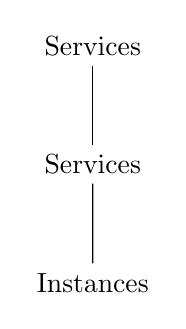
\begin{tikzpicture}
    \node [rectangle] {Services} 
    child {node [rectangle] {Services}
    child {node [rectangle] {Instances}}};
  \end{tikzpicture}
  \caption{Cloud layers}
\end{figure}

The figure above, Figure 1, show the different layers that CloudML can and should support. 
The top most level is services that a provider might support, such as CDN, geo-based serving, monitoring and load balancing. 
All in all services that are external from customers actual application, but that can influence or monitor it.
The next level is software, this is for any software that are co-existing with or for the customers application, 
such as databases, application servers, logging services. All in all software that are running on the same instance as the application, 
but that the customer would like to have automatically or semi-automatically configured and reconfigured.
On the bottom there are two levels, both representing instances. In the instance-level CloudML should bind together instances 
such as different virtual machines. This level is tightly connected to the Software-layer as connections between instances 
is very likely to be defined through software, such as \index{databases}, web accelerators and application servers.
